\documentclass[10pt,A4]{article}

\usepackage[utf8]{inputenc}

\usepackage{xifthen}

\usepackage[thin]{roboto}

% set font default
\renewcommand*\familydefault{\sfdefault} 	
\usepackage[T1]{fontenc}

% more font size definitions
\usepackage{moresize}

\usepackage{hyperref}

%----------------------------------------------------------------------------------------
%	PAGE LAYOUT  DEFINITIONS
%----------------------------------------------------------------------------------------

%debug page outer frames
%\usepackage{showframe}			


%define page styles using geometry
\usepackage[a4paper]{geometry}		

% for example, change the margins to 2 inches all round
\geometry{top=1.75cm, bottom=-.6cm, left=1.5cm, right=1.5cm} 	

%use customized header
\usepackage{fancyhdr}				
\pagestyle{fancy}

%less space between header and content
\setlength{\headheight}{-5pt}		


%customize entries left, center and right
\lhead{}
\chead{ \small{Martin TOUZOT  $\cdot$ Ingénieur Généraliste en informatique $\cdot$  Chaville, France  $\cdot$  \textcolor{sectcol}{\textbf{martin.touzot@gmail.com}}  $\cdot$ +33 6 40 40 63 21}}
\rhead{}


%indentation is zero
\setlength{\parindent}{0mm}

%----------------------------------------------------------------------------------------
%	TABLE /ARRAY DEFINITIONS
%---------------------------------------------------------------------------------------- 

%for layouting tables
\usepackage{multicol}			
\usepackage{multirow}

%extended aligning of tabular cells
\usepackage{array}

\newcolumntype{x}[1]{%
>{\raggedleft\hspace{0pt}}p{#1}}%


%----------------------------------------------------------------------------------------
%	GRAPHICS DEFINITIONS
%---------------------------------------------------------------------------------------- 

%for header image
\usepackage{graphicx}

%for floating figures
\usepackage{wrapfig}
\usepackage{float}
%\floatstyle{boxed} 
%\restylefloat{figure}

%for drawing graphics		
\usepackage{tikz}				
\usetikzlibrary{shapes, backgrounds,mindmap, trees}


%----------------------------------------------------------------------------------------
%	Color DEFINITIONS
%---------------------------------------------------------------------------------------- 

\usepackage{color}

%accent color
\definecolor{sectcol}{RGB}{0,150,255}

%dark background color
\definecolor{bgcol}{RGB}{110,110,110}

%light background / accent color
\definecolor{softcol}{RGB}{0,225,225}


%============================================================================%
%
%
%	DEFINITIONS
%
%
%============================================================================%

%----------------------------------------------------------------------------------------
% 	HEADER
%----------------------------------------------------------------------------------------

% remove top header line
\renewcommand{\headrulewidth}{0pt} 

%remove botttom header line
\renewcommand{\footrulewidth}{0pt}	  	

%remove pagenum
\renewcommand{\thepage}{}	

%remove section num		
\renewcommand{\thesection}{}			

%----------------------------------------------------------------------------------------
% 	ARROW GRAPHICS in Tikz
%----------------------------------------------------------------------------------------

% a six pointed arrow poiting to the left
\newcommand{\tzlarrow}{(0,0) -- (0.2,0) -- (0.3,0.2) -- (0.2,0.4) -- (0,0.4) -- (0.1,0.2) -- cycle;}	

% include the left arrow into a tikz picture
% param1: fill color
%
\newcommand{\larrow}[1]
{\begin{tikzpicture}[scale=0.58]
	 \filldraw[fill=#1!100,draw=#1!100!black]  \tzlarrow
 \end{tikzpicture}
}

% a six pointed arrow poiting to the right
\newcommand{\tzrarrow}{ (0,0.2) -- (0.1,0) -- (0.3,0) -- (0.2,0.2) -- (0.3,0.4) -- (0.1,0.4) -- cycle;}

% include the right arrow into a tikz picture
% param1: fill color
%
\newcommand{\rarrow}
{
\begin{tikzpicture}[scale=0.7]
	\filldraw[fill=sectcol!100,draw=sectcol!100!black] \tzrarrow
 \end{tikzpicture}
}



%----------------------------------------------------------------------------------------
%	custom sections
%----------------------------------------------------------------------------------------

% create a coloured box with arrow and title as cv section headline
% param 1: section title
%
\newcommand{\cvsection}[1]
{
\colorbox{sectcol}{\mystrut \makebox[1\linewidth][l]{
\larrow{bgcol} \hspace{-8pt} \larrow{bgcol} \hspace{-8pt} \larrow{bgcol} \textcolor{white}{\textbf{#1}}\hspace{4pt}
}}\\
}

%create a coloured arrow with title as cv meta section section
% param 1: meta section title
%
\newcommand{\metasection}[2]
{
\begin{tabular*}{1\textwidth}{p{2.4cm} p{11cm}}
\larrow{bgcol}	\normalsize{\textcolor{sectcol}{#1}}&#2\\[12pt]
\end{tabular*}
}

%----------------------------------------------------------------------------------------
%	 CV EVENT
%----------------------------------------------------------------------------------------

% creates a stretched box as cv entry headline followed by two paragraphs about 
% the work you did
% param 1:	event time i.e. 2014 or 2011-2014 etc.
% param 2:	event name (what did you do?)
% param 3:	institution (where did you work / study)
% param 4:	what was your position
% param 5:	some words about your contributions
%
\newcommand{\cveventlong}[6]
{
\vspace{8pt}
	\begin{tabular*}{1\textwidth}{p{2.3cm}  p{10.8cm} x{3.9cm}}
 \textcolor{bgcol}{#1}& \textbf{#2} & \vspace{2.5pt}\textcolor{sectcol}{#3}

	\end{tabular*}
\vspace{-12pt}
\textcolor{softcol}{\hrule}
\vspace{6pt}
	\begin{tabular*}{1\textwidth}{p{2.3cm} p{14.4cm}}
&		 \larrow{bgcol}  #4\\[3pt]
&		 \larrow{bgcol}  #5\\[6pt]
&		 \larrow{bgcol}  #6\\[6pt]
	\end{tabular*}

}

\newcommand{\cvevent}[5]
{
\vspace{8pt}
	\begin{tabular*}{1\textwidth}{p{2.3cm}  p{10.8cm} x{3.9cm}}
 \textcolor{bgcol}{#1}& \textbf{#2} & \vspace{2.5pt}\textcolor{sectcol}{#3}

	\end{tabular*}
\vspace{-12pt}
\textcolor{softcol}{\hrule}
\vspace{6pt}
	\begin{tabular*}{1\textwidth}{p{2.3cm} p{14.4cm}}
&		 \larrow{bgcol}  #4\\[3pt]
&		 \larrow{bgcol}  #5\\[6pt]
	\end{tabular*}

}

\newcommand{\cveducation}[4]
{
\vspace{8pt}
	\begin{tabular*}{1\textwidth}{p{2.3cm}  p{8.8cm} x{5.9cm}}
 \textcolor{bgcol}{#1}& \textbf{#2} & \vspace{0.5pt}\textcolor{sectcol}{#3}

	\end{tabular*}
\vspace{-12pt}
\textcolor{softcol}{\hrule}
\vspace{6pt}
	\begin{tabular*}{1\textwidth}{p{2.3cm} p{14.4cm}}
&		 \larrow{bgcol}  #4\\[3pt]
	\end{tabular*}

}

% creates a stretched box as 
\newcommand{\cveventmeta}[2]
{
	\mbox{\mystrut \hspace{87pt}\textit{#1}}\\
	#2
}

%----------------------------------------------------------------------------------------
% CUSTOM STRUT FOR EMPTY BOXES
%----------------------------------------- -----------------------------------------------
\newcommand{\mystrut}{\rule[-.3\baselineskip]{0pt}{\baselineskip}}


%============================================================================%
%
%
%
%	DOCUMENT CONTENT
%
%
%
%============================================================================%
\begin{document}


%use our custom fancy header definitions
\pagestyle{fancy}	


%---------------------------------------------------------------------------------------
%	TITLE HEADLINE
%----------------------------------------------------------------------------------------
\vspace{-20.55pt}

% use this for multiple words like working titles etc.
%\hspace{-0.25\linewidth}\colorbox{bgcol}{\makebox[1.5\linewidth][c]{\hspace{46pt}\HUGE{\textcolor{white}{\textsc{Jan Küster}} } \textcolor{sectcol}{\rule[-1mm]{1mm}{0.9cm}} \parbox[b]{5cm}{   \large{ \textcolor{white}{{IT Consultant}}}\\
% \large{ \textcolor{white}{{Resume}}}}
%}}

% use this for single words, e.g. CV or RESUME etc.
\hspace{-0.25\linewidth}\colorbox{bgcol}{\makebox[1.5\linewidth][c]{\HUGE{\textcolor{white}{\textsc{Martin TOUZOT}} } \textcolor{sectcol}{\rule[-1mm]{1mm}{0.9cm}} \HUGE{\textcolor{white}{\textsc{Curriculum vitæ}} } }}


%----------------------------------------------------------------------------------------
%	HEADER IMAGE
%----------------------------------------------------------------------------------------

\begin{figure}[H]
\begin{flushright}
	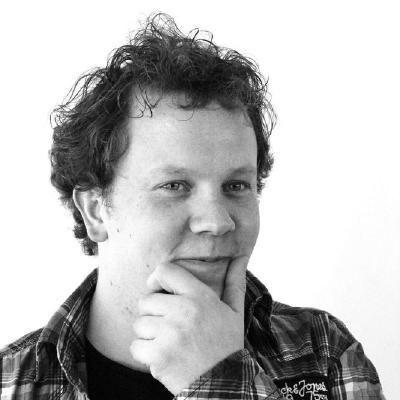
\includegraphics[clip,width=0.2\linewidth]{resume/profil_picture.jpg}	%trimming relative to image size!
\end{flushright}
\end{figure}

%---------------------------------------------------------------------------------------
%	META SECTION
%----------------------------------------------------------------------------------------

\vspace{-114pt}

\metasection{Informatique:}{Python, C, C++, Git, Qt, OpenCV, Linux, Windows}
\metasection{Langues:}{Français, anglais (courant), espagnole (scolaire)}
\metasection{Caractère:}{Autonome, curieux, persévérant}
\metasection{Hobbies:}{Cinéma, lecture, course à pied, voyages, jeux de sociétés}

\vspace{6pt}

\cvsection{À propos de moi}\\
Diplômé de Télécom Physique Strasbourg, après quelques années d'expériences dans différentes structures, je souhaite aujourd'hui mettre à profit mes connaissances en informatique pour résoudre de nouveaux défis en traitement d'images.

\vspace{6pt}

%============================================================================%
%
%	CV SECTIONS AND EVENTS (MAIN CONTENT)
%
%============================================================================%

%---------------------------------------------------------------------------------------
%	EXPERIENCE
%----------------------------------------------------------------------------------------
\cvsection{Expérience}

%
\cveventlong{2019 - en cours}{Ingénieur R\&D informatique}{Parifex, Viroflay (78)}{Intégrations et tests des logiciels sur les systèmes de contrôle de vitesse}{Développement en Python d'algorithmes de traitement d'images et de données 3D LIDAR}{Obtention du certificat Sauveteur Secouriste du Travail (SST) en 2021 }

%\textcolor{softcol}{\hrule}

%
\cveventlong{2017 - 2019}{Ingénieur en informatique}{Intitek, Paris (75)}{\textsl{Valeo Vision, Bobigny (93)}: développement d'une application en C++/Qt d'analyses d'optiques automobiles}{\textsl{Michelin, Clermont-Ferrand (63)}: développement d'applications en C++/Qt, Matlab et C\# d'analyses et de gestions de données métiers autour du pneus}{\textsl{Solystic, Bagneux (75)}: étude et développement d'un algorithme de traitement d'images en Python \& C permettant d'apparier des plis postaux}


%\textcolor{softcol}{\hrule}

%
\cveducation{2016}{Projet de fin d'études}{ONERA, Palaiseau (91)}{Étude d'une méthode de suivi de particules en vélocimétie 3D par imagerie sous Matlab}


%---------------------------------------------------------------------------------------
%	EDUCATION SECTION
%--------------------------------------------------------------------------------------
\cvsection{Éducation}

\cveducation{2012 - 2016}{Ingénieur généraliste}{Télécom Physique Strasbourg, Illkirch-Graffestaden (67)}{Spécialité suive en dernière année : Acquisition et Traitement d'images}

%\textcolor{softcol}{\hrule}

%
\cveducation{2009 - 2012}{Classe Préparatoire }{Lycée Lalande, Bourg-en-Bresse (01)}{Classes Préparatoires aux Grandes Écoles (CPGE) Option Physique Chimie (PC)}

\cvsection{Activité extra-professionnelles}

\cveventlong{}{Associatif}{}{2023 - en cours : Secrétaire du Potager des Vignes de Parifex, création et gestion d'un potager d'entreprise}{2017 - 2023 : Membre de l'Association des Anciens Elèves de Télécom Physique Strasbourg, communication auprès du réseaux étudiants \& des anciens élèves, rédactions de lettres d'informations}{2013 - 2014 : Président du Club Cinéma de Télécom Physique Strasbourg, projection et débats autour du cinéma}

\cvevent{}{GitHub}{\href{https://github.com/mtouzot/}{github.com/mtouzot}}{\href{https://github.com/mtouzot/PapibotPi}{PapibotPi}: Bot Twitter codé en Python publiant des citations de manière automatique}{\href{https://mtouzot.github.io/GameBEye/}{GameBEye}: Librairie Python de traitement d'images de GameBoy Camera}

%-------------------------------------------------------------------------------------------------
%	ARTIFICIAL FOOTER (fancy footer cannot exceed linewidth) 
%--------------------------------------------------------------------------------------------------

\null
\vspace*{\fill}
\hspace{-0.25\linewidth}\colorbox{bgcol}{\makebox[1.5\linewidth][c]{\mystrut \small \textcolor{white}{\href{https://mtouzot.github.io/}{mtouzot.github.io}} \qquad \textcolor{white}{\href{https://www.linkedin.com/in/martintouzot/}{linkedin.com/in/martintouzot}}}}




%============================================================================%
%
%
%
%	DOCUMENT END
%
%
%
%============================================================================%
\end{document}
